% lagrangian-products.tex — \input'd from experiments/experiments.tex
%
% Lagrangian products of rotated 2D polygons: systematic search for
% Viterbo counterexamples in the space of Lagrangian products.
%
% Sources:
%   - Generated data: experiments/data/{pentagon_sweep,polygon_grid,random_products}.jsonl
%   - HK-O 2024 counterexample: Haim-Kislev & Ostrover, Annals 2024
%   - Symmetry analysis: agent-written, Jörn-confirmed direction
%
% Structure:
%   - Mathematical setup (Lagrangian products, rotation parameter)
%   - Symmetry lemma (fundamental domain)
%   - Pentagon rotation curve (Family 1)
%   - Regular polygon grid (Family 2)
%   - Random Lagrangian products (Family 3)
%   - Findings

\subsection{Lagrangian Products of Rotated Polygons}
\label{sec:lagrangian-products}

The only known 4D counterexample to Viterbo's conjecture is a Lagrangian
product of two pentagons (Haim-Kislev \& Ostrover 2024). Random 4-polytopes
(Section~\ref{sec:systolic-ratios}) never exceeded~$\mathrm{sys} = 0.68$, far
below the Viterbo threshold. We probe the conjecture by searching
systematically in the space of Lagrangian products, where counterexamples are
known to exist.

\subsubsection*{Mathematical setup}

\begin{definition}[Lagrangian product]
\label{def:lagrangian-product}
Let~$P \subset \mathbb{R}^2_{q}$ and~$Q \subset \mathbb{R}^2_{p}$ be convex
polygons containing the origin. Their \emph{Lagrangian product} is
\[
  P \times_L Q
  \;=\; \bigl\{\, (q, p) \in \mathbb{R}^4 \;\big|\; q \in P,\; p \in Q \,\bigr\}
  \;\subset\; \mathbb{R}^4.
\]
The subspaces~$\mathbb{R}^2_q = \{(q_1, q_2, 0, 0)\}$
and~$\mathbb{R}^2_p = \{(0, 0, p_1, p_2)\}$ are both Lagrangian with respect
to~$\omega_0$.
\end{definition}

% [TODO: JÖRN - verify this volume claim. Standard but worth checking
%  the normalization factor: vol_4 vs 4D Lebesgue measure.]
The 4-volume satisfies~$\operatorname{vol}_4(P \times_L Q)
= \operatorname{area}(P) \cdot \operatorname{area}(Q)$ (Fubini's theorem on
complementary subspaces). Since volume factors, the systolic ratio becomes
\[
  \mathrm{sys}(P \times_L Q)
  \;=\; \frac{c_{\mathrm{EHZ}}(P \times_L Q)^2}
             {2 \,\operatorname{area}(P) \cdot \operatorname{area}(Q)}.
\]

\paragraph{Rotation parameter.}
Fix a polygon~$P$ in $q$-space. For an angle~$\theta$, let~$R(\theta)$ denote
the standard rotation in~$\mathbb{R}^2$ and
define~$Q_\theta = R(\theta)\,Q$. We study the one-parameter family
\[
  K_\theta \;=\; P \times_L Q_\theta.
\]
Since rotating both factors by the same angle~$\varphi$ is a symplectic
transformation~$\operatorname{diag}(R(\varphi), R(\varphi)) \in \mathrm{Sp}(4)$,
only the \emph{relative} rotation between the factors affects~$\mathrm{sys}$.

\begin{lemma}[Scale invariance of sys]
\label{lem:sys-scale-invariant}
For any convex body~$K \subset \mathbb{R}^4$ with~$0 \in \operatorname{int}(K)$
and any~$\lambda > 0$:~$\mathrm{sys}(\lambda K) = \mathrm{sys}(K)$.
\end{lemma}

\begin{proof}
The EHZ capacity is 2-homogeneous:~$c_{\mathrm{EHZ}}(\lambda K)
= \lambda^2 \, c_{\mathrm{EHZ}}(K)$. The 4-volume is 4-homogeneous.
Hence~$\mathrm{sys}(\lambda K) = (\lambda^2 c)^2 / (2 \lambda^4 v)
= c^2 / (2v) = \mathrm{sys}(K)$.
\end{proof}

\begin{lemma}[Fundamental domain for rotation sweeps]
\label{lem:rotation-fundamental-domain}
Let~$P$ be a regular $n$-gon and~$Q$ a regular $m$-gon, both centered at the
origin. Then~$\mathrm{sys}(P \times_L Q_\theta)$ depends on~$\theta$ only
through its equivalence class in~$[0, \pi/\operatorname{lcm}(n,m)]$.
\end{lemma}

\begin{proof}
\emph{Periodicity.}
The block-diagonal matrix~$M_\varphi = \operatorname{diag}(R(\varphi),
R(\varphi))$ is symplectic (direct verification:~$M_\varphi^T J_0 M_\varphi
= J_0$). Applying~$M_{2\pi/n}$ to~$P \times_L Q_\theta$ maps~$P$ to itself
(by $n$-fold rotational symmetry) and replaces~$Q_\theta$
with~$Q_{\theta + 2\pi/n}$. Similarly, the $m$-fold symmetry of~$Q$ gives
$Q_\theta = Q_{\theta + 2\pi/m}$. The combined periodicity
is~$2\pi/\operatorname{lcm}(n,m)$.

\emph{Mirror symmetry.}
The matrix~$M = \operatorname{diag}(-1, 1, -1, 1)$ is symplectic
(verification:~$M^T J_0 M = J_0$). It acts on~$\mathbb{R}^2_q$ as reflection
across the~$q_2$-axis and on~$\mathbb{R}^2_p$ as reflection across
the~$p_2$-axis. For our angle convention (normals starting at~$\pi/2$), both
regular polygons are invariant under these reflections, and~$M$
maps~$Q_\theta$ to~$Q_{-\theta}$.

Together: $\mathrm{sys}(\theta)$ has period~$2\pi/\operatorname{lcm}(n,m)$ and
satisfies~$\mathrm{sys}(\theta) = \mathrm{sys}(-\theta)$, so the fundamental
domain is~$[0, \pi/\operatorname{lcm}(n,m)]$.
\end{proof}

\begin{remark}
For pentagon~$\times$~pentagon:
$\operatorname{lcm}(5,5)=5$, fundamental
domain~$[0^\circ, 36^\circ]$. The HK-O counterexample at~$90^\circ$
maps to~$90 \bmod 72 = 18^\circ$ in this domain.
\end{remark}

% [TODO: JÖRN - verify factor swap claim. Agent derived that N = -J_0
%  is symplectic and maps P x_L Q to Q x_L (-P). For centrally symmetric
%  polygons, swapping factors preserves sys. For odd polygons, -P = R(π)P
%  so the swap also rotates one factor by 180°.]

\subsubsection*{Family 1: Pentagon rotation curve}

We sweep~$\theta \in [0^\circ, 90^\circ]$ at~$0.25^\circ$ resolution (361
points) for the family~$\mathrm{Pentagon} \times_L R(\theta)\,\mathrm{Pentagon}$,
where each pentagon is regular with circumradius~1. Each EHZ capacity
computation takes approximately~2.5\,s (10 facets).

% [TODO: replace with actual figure once data is generated]
Figure~\ref{fig:pentagon-sweep} shows the resulting curve.

\begin{figure}[h]
\centering
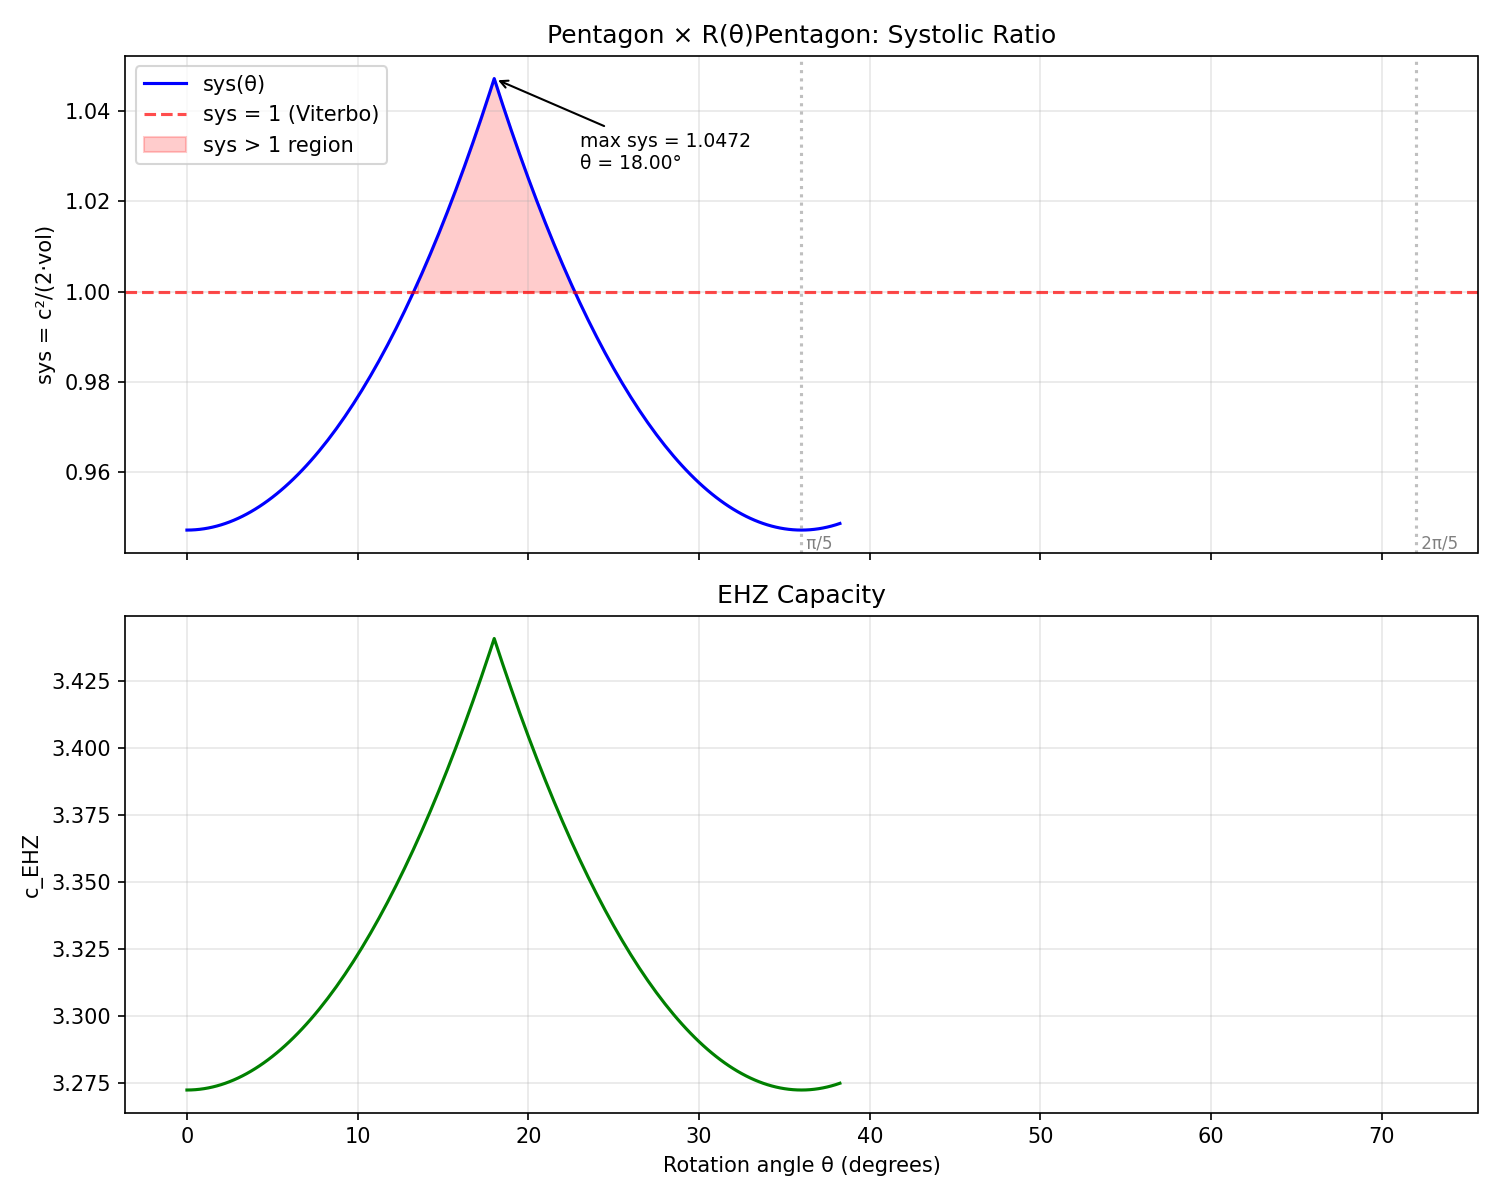
\includegraphics[width=0.9\textwidth]{../experiments/figures/pentagon_sweep.png}
\caption{Systolic ratio of $\mathrm{Pentagon} \times_L R(\theta)\,
  \mathrm{Pentagon}$ as a function of rotation angle~$\theta$. The red
  dashed line marks $\mathrm{sys} = 1$ (Viterbo threshold).}
\label{fig:pentagon-sweep}
\end{figure}

% [TODO: fill in findings after data is generated]

\subsubsection*{Family 2: Regular polygon pairs}

We sweep the rotation angle for all pairs~$(n, m)$ with~$3 \le n \le m$
and~$n + m \le 12$, sweeping~$\theta$ over the fundamental domain
$[0, \pi/\operatorname{lcm}(n,m)]$ at adaptive resolution (360 points for
$F \le 8$, down to~30 for $F = 12$).

\begin{figure}[h]
\centering
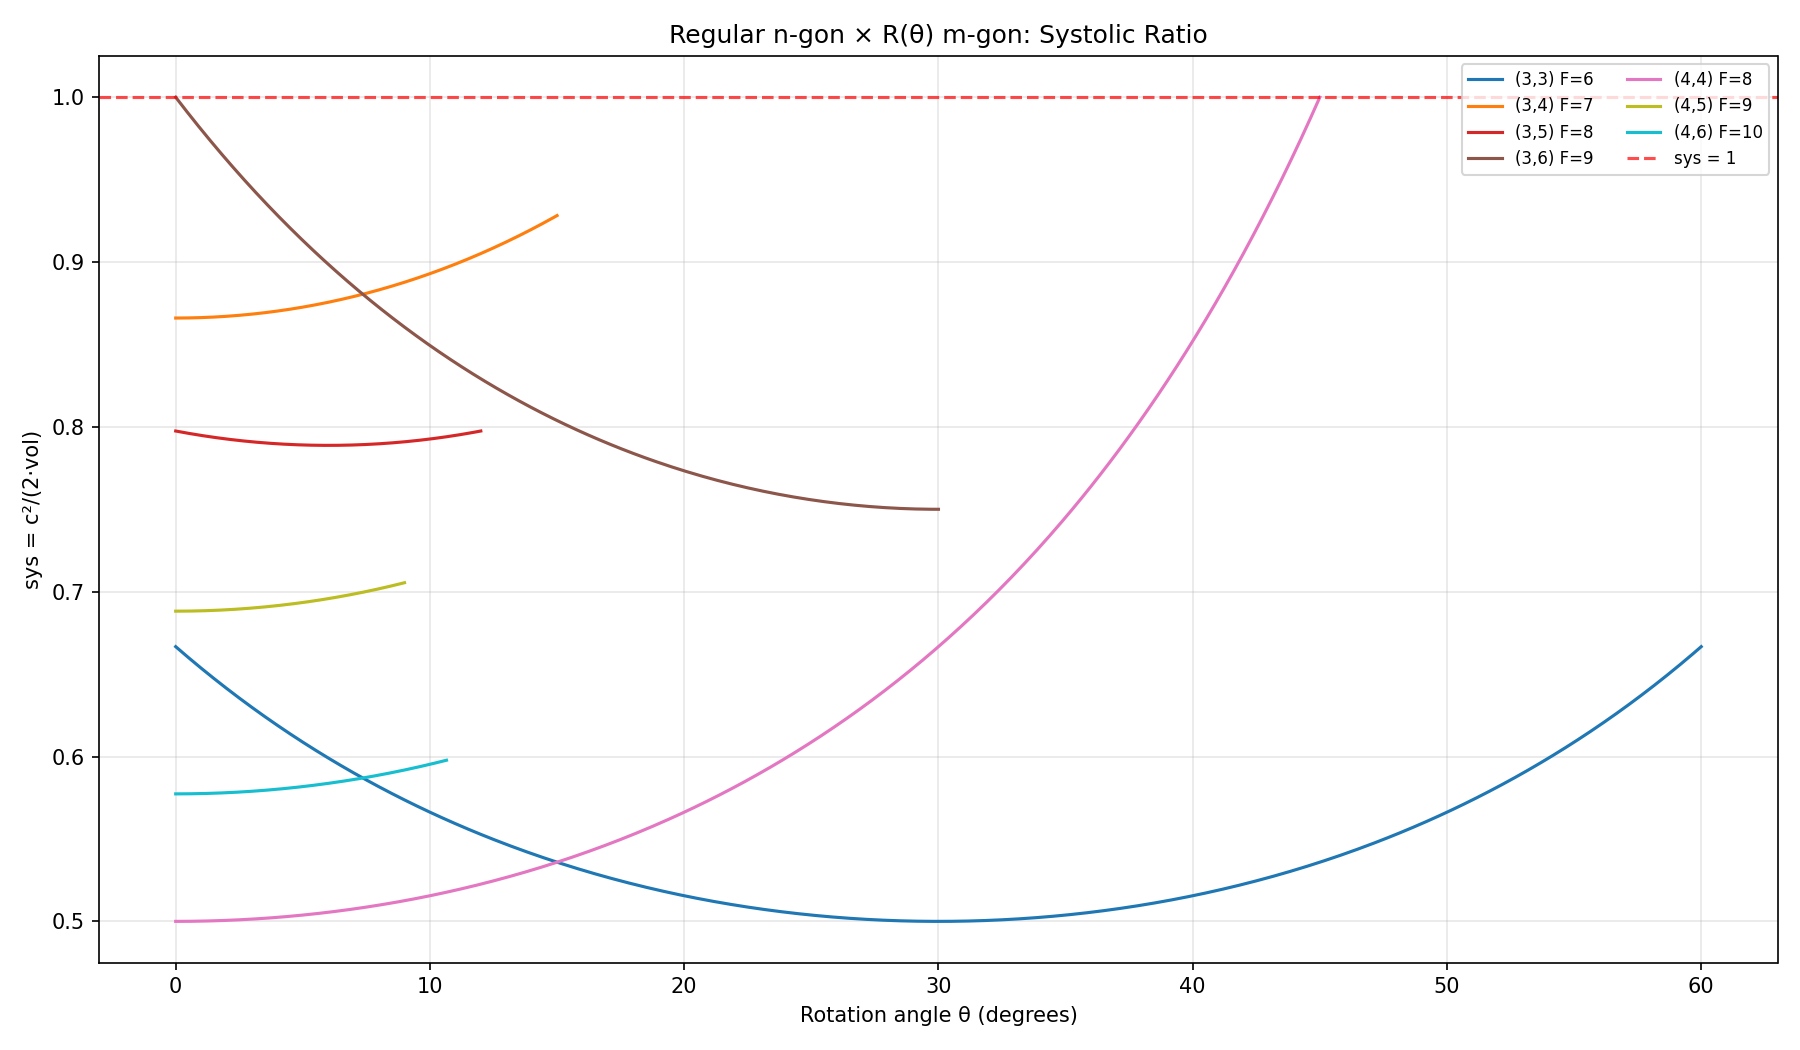
\includegraphics[width=0.9\textwidth]{../experiments/figures/polygon_grid.png}
\caption{Systolic ratio curves for regular $n$-gon $\times_L$ $R(\theta)$
  $m$-gon, for all pairs with $n + m \le 12$.}
\label{fig:polygon-grid}
\end{figure}

% [TODO: fill in summary table and findings after data is generated]

\subsubsection*{Family 3: Random Lagrangian products}

We generate 500 random Lagrangian products by sampling random convex
polygons (3--6 sides each, heights in~$[0.3, 2.0]$) and forming their
Lagrangian product. The rotation between factors is implicit in the random
orientations.

\begin{figure}[h]
\centering
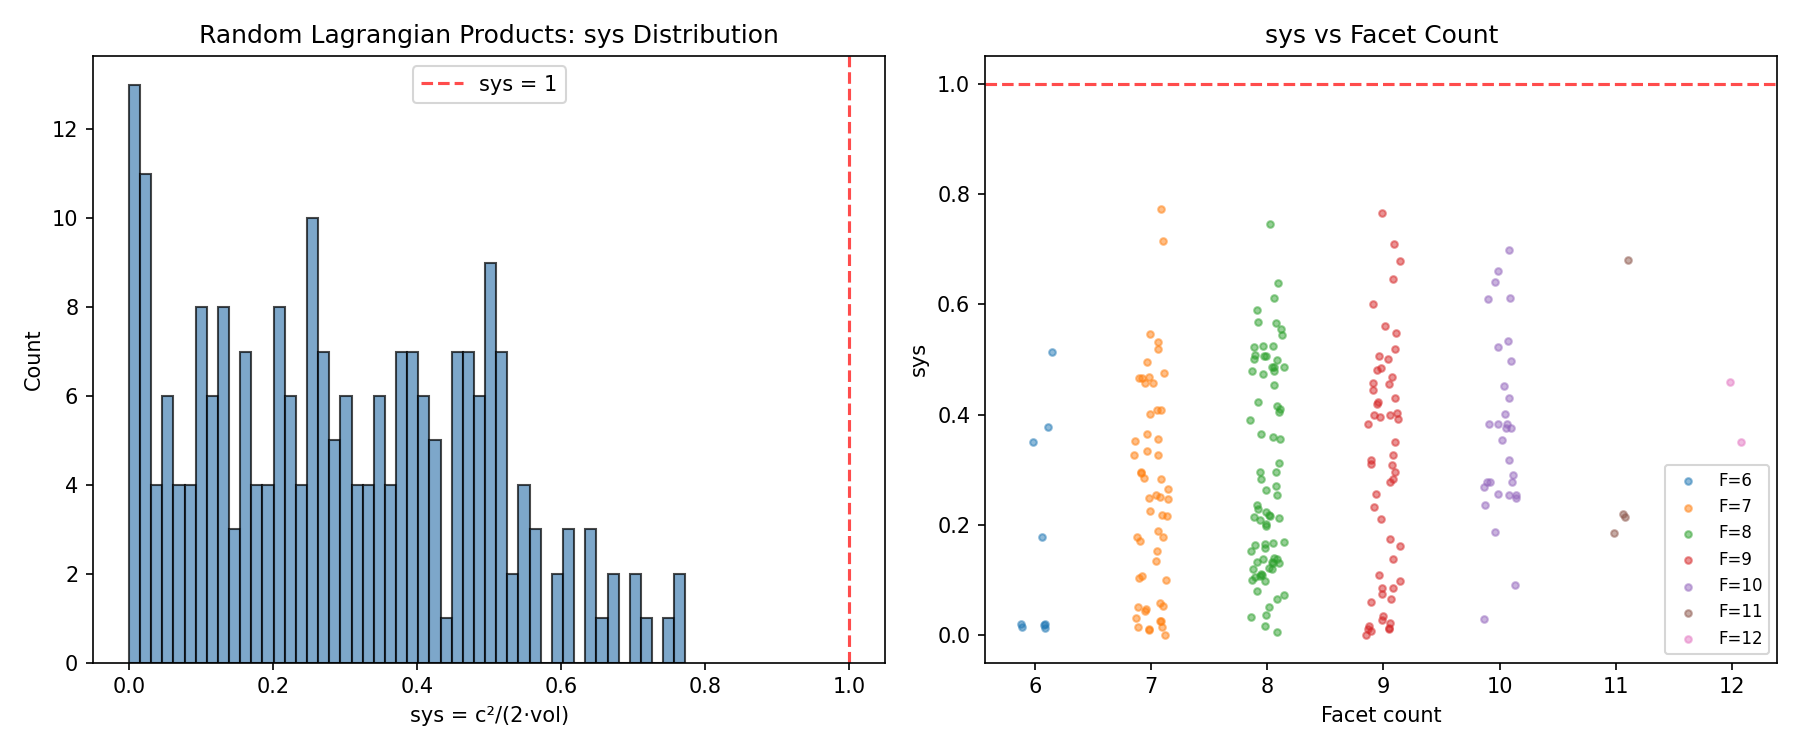
\includegraphics[width=0.9\textwidth]{../experiments/figures/random_products.png}
\caption{Distribution of systolic ratios for random Lagrangian products,
  compared with random (non-product) polytopes from
  Section~\ref{sec:systolic-ratios}.}
\label{fig:random-products}
\end{figure}

% [TODO: fill in findings after data is generated]

\subsubsection*{Findings}

% [TODO: write findings after all three families are computed.
%  Key questions to answer:
%  1. What does the pentagon curve look like? Where exactly is sys > 1?
%  2. Which other polygon pairs achieve sys > 1?
%  3. Do random Lagrangian products reach sys > 1?
%  4. What does this tell us about the prevalence of Viterbo violations?]
